To evaluate the behavior and accuracy of ConPaaS when hosting web applications, we prepared a realistic and complex enough scenario to assess any PaaS. In particular, we deployed the Wikipedia web application called MediaWiki~\cite{mediawiki}, and used a web hosting benchmark called WikiBench~\cite{wikibench}. 

%In this section, we describe our scenario in detail.

The architecture of the Wikipedia website uses a http-proxy, a http-web server, a database and one or more FPM-PhP web servers. To deploy it on ConPaaS, we composed two different services: the PHP web hosting and MySQL service. In the MySQL service, we installed a complete copy of English Wikipedia database which contains about 30GB in Wikipedia articles. In the PhP service, an initial configuration was composed of one Nginx HTTP-proxy, one Apache HTTP server, and one or more FPM-PhP (FastCGI Process Manager) servers. Each FPM-PhP server hosts the MediaWiki application which is the main component of this system. 

Since Wikipedia has a variable amount of data and visitors, it represents a valid example of elastic web applications. In this paper, we focus in the scalability of the PhP web hosting service, and thereby as the number of PhP servers hosting MediaWiki scale out or back based on the demanding workload.

In order to benchmark ConPaaS when hosting the Wikipedia services, we used the WikiBench research tool which generates realistic benchmarks with adaptable traffic properties. WikiBench has a number of advantages compared to the existing benchmark tools for web applications. First of all, Wikibench traces add a high degree of realism, since it is entirely based on the Wikipedia software and data. Indeed, the benchmark workloads are generated based on real access traces from the WikiMedia Foundation. These traces contain detailed  traffic logs of requests made to Wikipedia by its users. Since the original Wikipedia traces can reach peaks of 50000 or 60000 reqs./secs, WikiBench uses the original 10\% sample of these traces which can generate a workload up to about 5000 reqs./secs. As an example, in Figure~\ref{workload}, we show the workload of one trace as the number of request per minute during approximately 24h. 


% Similarly, the intensity of the resulting traffic could also be modified ranging from very low up to the 
% original traffic intensity of the trace. 

%Initial benchmark results show a typical day of Wikipedia traffic and the relation between the request rate %and the server response times. 


\begin{figure}
\begin{center}
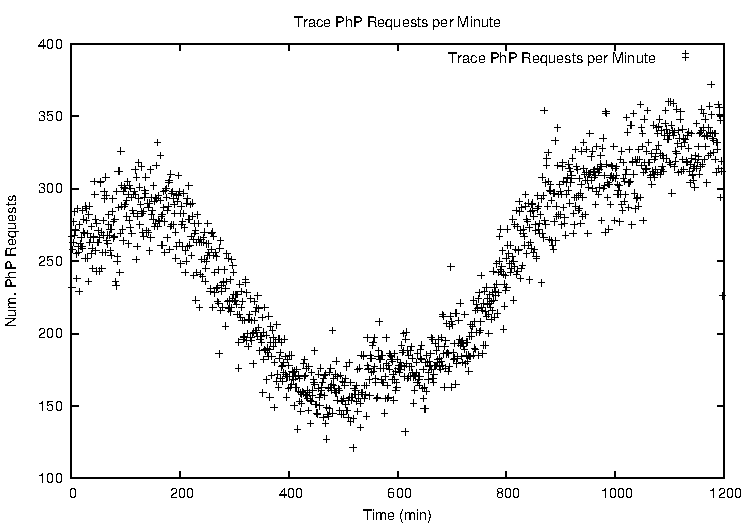
\includegraphics[width=0.49\textwidth, height=6cm]{./images/traceWorkload}
\end{center}
\caption{Wikipedia trace workload}
\label{workload}
\end{figure}

Even though we use a 10\% of the real traces, they are very heterogeneous regarding the type of user requests, and thus explaining the irregular performance pattern followed by web applications. 
We highlight the following properties that we consider important about these requests: 

\begin{itemize}
\item The intervarrival time between requests follows a Poisson distribution.

\item The distribution of page popularity varies from very popular pages to those following a Zipf distribution, and finally to a large part of them being accessed very infrequently.

\item The ratio of static/non-static file requestspresents a strong variation. Even though, most requests are for images, css and other static files. The types of requests are related, as the result of a Wikipedia web page includes images, css stylesheets and other static files. In particular, most web pages contains PhP code to be compiled that increases significantly the response time. We identify the reasons of this increment and we want to retain:

\begin{itemize}
\item PhP web pages often require DB queries.
\item PhP pages vary in complexity so it is difficult to make predictions.
\end{itemize}

\item The ratio of read/write operations vary having more reads than editions or creations of wiki pages.

\item A considerable amount of requests for non-existing pages and files, which obviously add realism to the traffic.

\end{itemize}


%By using real world server side software and data, we think the WikiBench benchmarking suite is a very  realistic and extensible research tool.

% these traces create workloads for WikiBench instead of creating purely synthetic workloads like other benchmarking tools have done.



